\chapter{Exceptions in programming languages}

``Exceptions'' is a broader term referring to a strategy of handling erroneous
states in computer programs by interrupting normal program execution, running special
code called an \emph{exception handler} and then resuming execution in a known, different
state.

The usual terminology is not very strict: the word ``exception'' may mean sligtly
different things -- or different sides of the same thing -- in different contexts.
For example, programming languages are said to \emph{have exceptions} if they support
this kind of error handling; exceptions are said to \emph{be compiled}, while it is the
corresponding infrastructure and support code that is compiled; often the word ``exception''
denotes a piece of information about the error being handled; et cetera.

When an error occurs during normal execution of a program, \emph{an exception is thrown}%
\footnote{Some programming languages, such as Python, use the term \emph{raised}.%
\cite{python:reference}}.
This starts the
process of \emph{handling the exception}: looking for a suitable
\emph{exception handler} that \emph{handles the exception}, either by \emph{catching} it
to resume normal computation, or by \emph{re-throwing} it to find another handler
able to deal with the error.

Due to common names of the corresponding syntactic features of popular programming languages%
\footnote{Most of them use the same keywords for this purpose.},
a piece of code together with attached pieces of handler code is called a \emph{try-block},
and a piece of handler code is called a \emph{catch-block}.

Most languages also provide \emph{finally-blocks}. These are pieces of code attached to a
try-block that are guaranteed to be executed after the try-block, whether an exception
has been thrown or not. Because of this property, finally-blocks are usually used to clean up
resources. In this thesis, we will not model finally-blocks as these can be
supplemented by an appropriate use of all-catching exception handlers.

There may be multiple handlers attached to a piece of code.
As already mentioned, the word ``exception'' also denotes a piece of information about
the error or condition causing the exceptional state, modeled by a value of the programming
language. In typed languages, these values have types, exception handlers declare what
types of exceptions they can handle, and based on the type of the thrown exception,
an appropriate handler is selected. The handler can then inspect the exception and
behave appropriately.

A try-block needn't have handlers for all exceptions that might arise within. If an exception
is \emph{uncaught} within a try-block, it is \emph{propagated} to the containing try-block,
which may not catch this exception as well, propagating it further.
If an exception propagates all the way out of all nested try-blocks, the program usually
aborts.

To give a quick illustration how try-blocks look in the concrete syntax of some widely used
languages, \Fref{fig:try-blocks} contains four examples.\footnote{Note that OCaml does not
have syntax for finally-blocks; these are simulated by a function. Haskell does not have
syntax for exceptions at all, both \emph{catch} and \emph{finally} are just functions.
All code snippets are just symbolic and have been stripped of non-relevant context, such
as library imports and the definitions of the functions \emph{perform\_work}
and \emph{do\_cleanup}.}

\begin{figure}
%
\begin{subfigure}[b]{0.46\textwidth}\begin{codepy}
try:
	perform_work()
except IOError:
	print "IO error caught"
finally:
	do_cleanup()
\end{codepy}\caption{Python}\end{subfigure}
%
\begin{subfigure}[b]{0.46\textwidth}\begin{codejava}
try {
	performWork();
} catch (IOException e) {
	System.out.println(
	    "IO error caught");
} finally {
	doCleanup();
}
\end{codejava}\caption{Java}\end{subfigure}

\begin{subfigure}[b]{0.46\textwidth}\begin{codehs}
performWork
 `catch` (\(e :: IOException) ->
   putStrLn "IO error caught")
 `finally` 
   doCleanup
\end{codehs}\caption{Haskell}\end{subfigure}
%
\begin{subfigure}[b]{0.46\textwidth}\begin{codeml}
finally do_cleanup (fun () ->
  try perform_work ()
  with IO_error ->
    print_string "IO error caught"
) ()
\end{codeml}\caption{OCaml}\end{subfigure}

\caption{Try-blocks in different languages}
\label{fig:try-blocks}
\end{figure}

\todo{Really include ``finally''? Revise OCaml.}

\section{Purpose}

As already mentioned, in practice, exceptions are mostly used to handle errors or
other exceptional states. The advantage to using
exceptions for this purpose is separation of concerns and hence cleaner resulting code.
Especially when reading a program, the reader first reads the code related the expected
execution path, uncluttered with error checks, which brings forward the main idea
of the code.

However, some languages, for example Python or OCaml, use exceptions also for control-flow
purposes, not only in rare critical events. Python iterators raise an exception to
indicate the end of stream \cite{python:reference}; also file-I/O functions in OCaml raise
an exception to indicate the end of file \cite{ocaml:reference}. The implementation of
exceptions in these languages is efficient enough to make them cheap and enable this approach.

\todo{Disadvantages. Multiple exit points, reasoning.}

\todo{Extend this section.}

\section{History}

Louden and Lambert describe the invention of exceptions in their book
\emph{Programming Languages: Principles and Practice} as follows.

\begin{quote}
Exception handling was pioneered by the language PL/I in the 1960s and
significantly advanced by CLU in the 1970s, with the major design questions
eventually resolved in the 1980s and early 1990s. Today, virtually all major
current languages, including C++, Java, Ada, Python, ML, and Common Lisp (but
not C, Scheme or Smalltalk) have built-in exception handling mechanisms.
Exception handling has, in particular, been integrated very well into
object-oriented mechanisms in Python, Java, and C++, and into functional
mechanisms in ML and Common Lisp. Also, languages that do not have built-in
mechanisms sometimes have libraries available that provide them, or have other
built-in ways of simulating them. \cite[p.~423]{louden:languages}
\end{quote}

% http://stackoverflow.com/questions/1449951/what-language-was-the-first-to-implement-exception-handling

\todo{Extend this section.}

\section{Theoretical appeal}

The theoretical appeal of exceptions in function languages is impossible to discuss
without having introduced the \emph{Curry-Howard correspondence}.

\subsection{The Curry-Howard correspondence}

The Curry-Howard correspondence establishes a relationship between typed programs and logic.
According to this interpretation, types of programs correspond to logical propositions --
and programs themselves correspond to proofs of logical propositions corresponding to their
types.

This correspondence goes all the way to relating whole $\lambda$-calculi to different
logical systems. For example, the simply typed $\lambda$-calculus corresponds to the minimal
logic, see \Fref{fig:stlc-ml}.

\begin{figure}
\centering
\begin{subfigure}[b]{0.45\textwidth}
\begin{prooftree}
\bax{$x : \sigma \in \Gamma$}
\bright{Ax}\bun{$\Gamma \vdash x : \sigma$}
\end{prooftree}
\begin{prooftree}
\bax{$\Gamma, x : \sigma \vdash M : \tau$}
\bright{Abstr}\bun{$\Gamma \vdash (\lambda x:\sigma. M) : \sigma \to \tau$}
\end{prooftree}
\begin{prooftree}
\bax{$\Gamma \vdash f : \sigma \to \tau$}
\bax{$\Gamma \vdash x : \sigma$}
\bright{App}\bbin{$\Gamma \vdash f x : \tau$}
\end{prooftree}

\caption{$\lambda_\to$}
\end{subfigure}
%
\begin{subfigure}[b]{0.45\textwidth}
\begin{prooftree}
\bax{$A \in \Gamma$}
\bright{Ax}\bun{$\Gamma \vdash A$}
\end{prooftree}
\begin{prooftree}
\bax{$\Gamma, A \vdash B$}
\bright{$I_\to$}\bun{$\Gamma \vdash A \to B$}
\end{prooftree}
\begin{prooftree}
\bax{$\Gamma \vdash A \to B$}
\bax{$\Gamma \vdash A$}
\bright{$E_\to$}\bbin{$\Gamma \vdash B$}
\end{prooftree}
\caption{$ML$}
\end{subfigure}

\caption{Simply typed $\lambda$-calculus ($\lambda_\to$), compared to minimal logic (ML).}
\label{fig:stlc-ml}
\end{figure}

When put side-by-side, it can be seen that the typing rules for the simply typed
$\lambda$-calculus become precisely the natural-deduction rules for minimal logic
if terms are erased and only types are retained.

In this interpretation, \emph{function application} on the computational side corresponds
to \emph{modus ponens} (or implication elimination) on the logic side, and
\emph{$\lambda$-abstraction} corresponds to the \emph{deduction theorem} (or implication
introduction).

The correspondence between certain $\lambda$-calculi and logic systems was presented
by Barendregt in \cite{barendregt91} in the elegant form of the $\lambda$-cube, as seen in
\Fref{fig:lambda-cube}. The names of the $\lambda$-calculi and the corresponding
logic systems are listed in \Fref{tab:lambda-cube}.

\begin{figure}
\centering
\begin{subfigure}{0.4\textwidth}
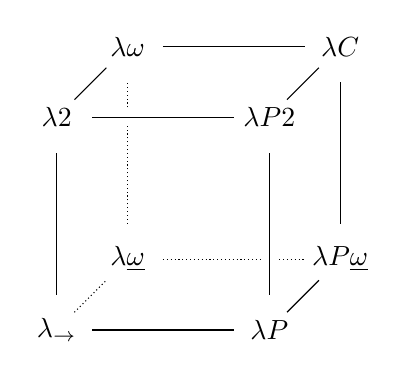
\begin{tikzpicture}[x=9mm,y=9mm,
        back line/.style={densely dotted,-},
        normal line/.style={-stealth,-},
        cross line/.style={normal line,-,
           preaction={draw=white, -, 
           line width=6pt}},
    ]
    \draw
    	(0,0) node{$\lambda_\to$}
    	(3,0) node{$\lambda{}P$}
    	(0,3) node{$\lambda{}2$}
    	(3,3) node{$\lambda{}P2$}
    	(1,1) node{$\lambda\underline{\omega}$}
    	(4,1) node{$\lambda{}P\underline{\omega}$}
    	(1,4) node{$\lambda\omega$}
    	(4,4) node{$\lambda{}C$}
	    ;
	\draw
		(1,1)
		+(0.5,0) edge[back line] +(2.5,0)
		+(0,0.5) edge[back line] +(0,2.5)
		+(0.5,3) edge[normal line] +(2.5,3)
		+(3,0.5) edge[normal line] +(3,2.5)
		;
	\draw[normal line]
		(0,0)
		+(0.5,0) edge +(2.5,0)
		+(0,0.5) edge +(0,2.5)
		+(0.5,3) edge[cross line] +(2.5,3)
		+(3,0.5) edge[cross line] +(3,2.5)
		;
	\draw
		(0,3) +(0.25,0.25) edge[normal line] +(0.7,0.7)
		(3,3) +(0.25,0.25) edge[normal line] +(0.7,0.7)
		(3,0) +(0.25,0.25) edge[normal line] +(0.7,0.7)
		(0,0) +(0.25,0.25) edge[back line] +(0.7,0.7)
		;
\end{tikzpicture}
\caption{$\lambda$-cube}
\end{subfigure}
%
\begin{subfigure}{0.4\textwidth}
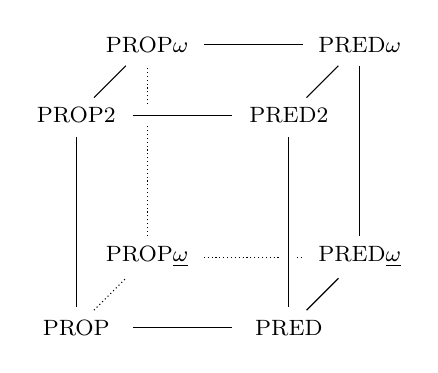
\begin{tikzpicture}[x=9mm,y=9mm,
        back line/.style={densely dotted,-},
        normal line/.style={-stealth,-},
        cross line/.style={normal line,-,
           preaction={draw=white, -, 
           line width=6pt}},
    ]
    \draw[font=\footnotesize]
    	(0,0) node{PROP}
    	(3,0) node{PRED}
    	(0,3) node{PROP2}
    	(3,3) node{PRED2}
    	(1,1) node{PROP$\underline{\omega}$}
    	(4,1) node{PRED$\underline{\omega}$}
    	(1,4) node{PROP$\omega$}
    	(4,4) node{PRED$\omega$}
	    ;
	\draw
		(1,1)
		+(0.8,0) edge[back line] +(2.2,0)
		+(0,0.3) edge[back line] +(0,2.7)
		+(0.8,3) edge[normal line] +(2.2,3)
		+(3,0.3) edge[normal line] +(3,2.7)
		;
	\draw[normal line]
		(0,0)
		+(0.8,0  ) edge +(2.2,0  )
		+(0  ,0.3) edge +(0  ,2.7)
		+(0.8,3  ) edge[cross line] +(2.2,3  )
		+(3  ,0.3) edge[cross line] +(3  ,2.7)
		;
	\draw
		(0,3) +(0.25,0.25) edge[normal line] +(0.7,0.7)
		(3,3) +(0.25,0.25) edge[normal line] +(0.7,0.7)
		(3,0) +(0.25,0.25) edge[normal line] +(0.7,0.7)
		(0,0) +(0.25,0.25) edge[back line] +(0.7,0.7)
		;
\end{tikzpicture}
\caption{Logic-cube}
\end{subfigure}
%
\caption{The $\lambda$-cube and the corresponding logic-cube \cite{barendregt91}}
\label{fig:lambda-cube}
\end{figure}

\begin{table}
\centering
\begin{tabular}{lll}
\toprule
\textit{$\lambda$-calculus} & \textit{logic} & \textit{description} \\
\midrule
$\lambda_\to$ & PROP & first-order propositional \\
$\lambda{}P$ & PRED & first-order predicate \\
$\lambda{}2$ & PROP2 & second-order propositional \\
$\lambda{}P2$ & PRED2 & second-order predicate \\
$\lambda\underline{\omega}$ & PROP$\underline{\omega}$ & weakly higher-order propositional \\
$\lambda{}P\underline{\omega}$& PRED$\underline{\omega}$ & weakly higher-order predicate \\
$\lambda\omega$ & PROP$\omega$ & higher-order propositional \\
$\lambda{}C$ & PRED$\omega$ & higher-order predicate \\
\bottomrule
\end{tabular}

\vspace{8pt}
{\small The calculus $\lambda_\to$ is also called the \emph{simply typed $\lambda$-calculus} (STLC)
and the calculus $\lambda{}C$ is also called the \emph{calculus of constructions} (CoC).}
\caption{The $\lambda$-calculi and logic systems of the $\lambda$-cube \cite{barendregt91}}
\label{tab:lambda-cube}
\end{table}

\todo{Talk about dependent types, Coq, proving, Type theory, \ldots ?}

\subsection{Control operators}

In functional languages, exceptions are closely related to the theory of
\emph{control operators}\footnote{Such as \ident{call/cc} in Scheme.},
for example the calculus $\lC$ introduced by Felleisen in \cite{felleisen87}
as a way to reason about abortive programs. An accessible formal description
thereof can be found in \cite[p.~876, Section~3]{ariola-herbelin} or
\cite{griffin90}; here we will restrict ourselves to an informal sketch.

Felleisen introduced three control operators, $\bigC$ for ``control'', $\bigA$
for ``abort'', and $\bigK$, representing \ident{call/cc}. The operator $\bigA$ \emph{aborts}:
takes a value and replaces the current context with it; the operator $\bigK$
takes a function and applies it to the current context (reified as a continuation),
and finally the operator $\bigC$ takes a function and replaces the current context
with the function applied to the original context, thus being a combination of
the former two; an overview can be seen in \Fref{tab:control-operators}.

\begin{table}[htp]
\centering
\begin{tabular}{llll}
\toprule
\thead{Operator} & \thead{Replaces CC*} & \thead{Provides CC**} & \thead{In terms of the others} \\
\midrule
$\bigC$ & yes & yes & $\lambda M.\,\bigK(\lambda k.\,\bigA (M k))$\\
$\bigK$ & no & yes & $\lambda M.\,\bigC(\lambda k.\,k (M k)) $ \\
$\bigA$ & yes & no & $\lambda M.\,\bigC(\lambda \_.\,M)$ \\
\bottomrule
\end{tabular}

\vspace{2pt}
{\small *Current context. **Applies its argument to the current continuation.}
\caption{Overview of control operators}
\label{tab:control-operators}
\end{table}

The behavior of these operators is best shown on an example.

\subsubsection{Control operators and Curry-Howard}

In 1990, Griffin showed \cite{griffin90} that the control operator $\mathcal{C}$
used in $\lC$ can be given the type $\neg \neg A \to A$, yielding a \emph{computational
interpretation} of classical logic. However, this calculus did not match
classical natural deduction operationally \cite{ariola-herbelin}.

\todo{$\bigA$ is EFQ, $\bigC$ is DN, $\bigK$ is PL. DN implies everything ($\bigC$
subsumes the other two) and EFQ+PL implies DN (as $\bigC$ is definable from $\bigA$
and $\bigK$).}

From the other direction, Parigot created the $\lambda_\mu$ calculus \cite{parigot92}
as a way to assign computational content to classical natural deduction. The calculus
$\lambda_\mu$ Parigot presented did not readily correspond to classical logic --
only to minimal classical logic -- but it
can be extended to do so, finally yielding a calculus matching classical natural deduction
\cite{ariola-herbelin}.

\todo{Hence, control operators extend our logic up to classical logic!}

\subsection{Exceptions and control operators}

\todo{(Statically-bounded) exceptions can be implemented using control operators.}

\todo{Not the same, dynamic vs. static scoping \cite{thielecke:contrast, kameyama:dynamic}.}

\todo{With fresh variables, Peirce can be done.}

\section{Practical appeal}

\todo{Appeal of certified compilers.}

\label{chap:dependent-types}






































































